\documentclass[12pt,a4paper,fancyheader]{scrartcl}

\usepackage[ngerman]{babel}
\usepackage[utf8]{inputenc}
\usepackage{fancyhdr}
\usepackage{graphicx}
\usepackage{hyperref}
\usepackage{amsfonts}

\newcommand\svthema{ShroomScout}
\newcommand\svperson{Tim Hofmann, Lauritz Kremzow}
\newcommand\svdatum{\today}
\newcommand\lvname{Modul: Web Technologie}
\newcommand\lvtyp{WS 2023}
\newcommand\lvinst{FOM Hochschule für Oekonomie \& Management}

\hypersetup{
pdftitle={Seminararbeit zum Thema: \svthema} 
pdfauthor={\svperson}
}	
	
\begin{document}

\title{ \huge\textbf{\svthema} }
\author{ \textsl{\svperson} \\ \svdatum }
\date{ \normalsize \centering 
\includegraphics[width=0.3\textwidth]{abbildungen/FOM.jpg}\\\textsc{"`\lvname"'} \\ {\lvtyp} · {\lvinst} }

\maketitle
\thispagestyle{empty}
\pagenumbering{Roman}

\cleardoublepage
\tableofcontents
\cleardoublepage
\listoffigures
\cleardoublepage
\pagenumbering{arabic}
\setcounter{page}{4}

\documentclass[../main.tex]{subfiles} % ~1000 Worte

\begin{document}

\subsection{Motivation \& Zielbeschreibung} % Lauritz

Die Entwicklung von `ShroomScout', einer Webanwendung auf Angular-Basis, entspringt einer tiefen Leidenschaft
für das Pilzesammeln. Diese Freizeitbeschäftigung verbindet die Freude am Erkunden der Natur mit dem praktischen
Nutzen der Ernte essbarer Pilze aus ihrem natürlichen Umfeld. Die Erkenntnis, dass Pilze unter bestimmten Bedingungen
gedeihen und recht zuverlässig an denselben Stellen wiederkehren, motivierte zur Schaffung einer digitalen Plattform,
welche die Kartierung und gemeinschaftliche Nutzung von Pilzfundorten ermöglichen soll.

`ShroomScout' bedient sich einer interaktiven, auf OpenStreetMap basierten Karte, um Nutzern eine visuelle
Grundlage zum Eintragen der Standorte ihrer Pilzfunde bieten zu können. Die Benutzeroberfläche ist intuitiv gestaltet:
Mit einem einfachen Klick auf die Schaltfläche `Pilz eintragen' öffnet sich ein Eingabefenster, das nicht nur die
Eingabe des Pilznamens mittels automatischer Vervollständigung ermöglicht, sondern auch die Beschreibung der Umgebung,
in der der Pilz gefunden wurde. Ein visuelles Element in Form eines Bildes des Pilzes unterstützt den Nutzer dabei,
die korrekte Identifikation sicherzustellen, was besonders bei der Unterscheidung von essbaren und potenziell giftigen
Pilzen von unschätzbarem Wert ist.

Die Kernfunktionalität von `ShroomScout' wird durch einen Live-Feed ergänzt, der es den Nutzern ermöglicht,
in Echtzeit zu sehen, welche Pilze kürzlich und wo gefunden wurden. Diese Funktion fördert nicht nur den
Austausch innerhalb der Pilzsammlergemeinschaft, sondern trägt auch dazu bei, das Bewusstsein und das
Interesse am Pilzesammeln zu steigern --- eine Praxis, die in der heutigen Zeit vielleicht nicht mehr so
verbreitet ist wie in der Vergangenheit.

Das übergeordnete Ziel von `ShroomScout' ist also das Schaffen einer Plattform, die Pilzsammler bei der Dokumentation
ihrer Funde unterstützt, die Sicherheit beim Sammeln erhöht und letztlich eine Gemeinschaft Gleichgesinnter
aufbaut. Dabei bietet die Applikation eine wertvolle Ressource, die es ermöglicht, basierend auf der kollektiven Erfahrung
und dem Wissen der Nutzer fundierte Entscheidungen über die Identität und Sicherheit von Pilzen zu treffen. Durch die
Bereitstellung einer solchen Plattform soll das Interesse und Wissen um das Pilzesammeln gefördert und somit einen Beitrag
zur Wiederbelebung dieser traditionellen Aktivität geleistet werden.

\subsection{Projektmethodik \& Herangehensweise} % Lauritz

Die Planungsphase des Projekts `ShroomScout' begann mit der Ideenfindung und der Identifikation essenzieller Use Cases,
die das Interagieren mit der Karte, das Eintragen eines Pilzes und die Verfolgung des Live-Feeds umfassten. Diese initialen
Überlegungen führten zur detaillierten Skizzierung aller Aspekte der grafischen Benutzeroberfläche (GUI), um einen klaren
Aufbau und eine intuitive Nutzerführung sicherzustellen. Die Planung mündete in einem Architekturentwurf, der eine Dreiteilung
in Frontend, Backend und eine Datenbank für die Speicherung der Koordinaten der eingetragenen Pilze vorsah. Nach Festlegung
dieser Struktur erfolgte die Auswahl der Technologien: Angular für das Frontend, um an vorhandene Kenntnisse anzuknüpfen,
FastAPI mit Python für das Backend, basierend auf positiven Erfahrungen in einem vorangegangenen Universitätsprojekt, und
SQLite als Datenbanklösung aufgrund ihrer Einfachheit und Effizienz.

Die Umsetzung des Projekts erfolgte nach agilen Prinzipien. Die Nutzung von GitHub ermöglichte eine effiziente Aufgabenverwaltung
auf einem Kanban-Board, wodurch eine kontinuierliche Entwicklung und Priorisierung von Features gewährleistet wurden. Tägliche
Abstimmungen im Rahmen von Daily Calls, angelehnt an die Scrum-Methodik, förderten die Kommunikation und Problemlösung im Team.
Der Einsatz von Git unterstützte die verteilte Entwicklung und sicherte einen reibungslosen Integrationsprozess der einzelnen
Komponenten. Die Arbeitsteilung erfolgte klar definiert in zum einen Frontend und zum anderen Backend/Datenbank, um an bisheriges
Wissen und individuelle Präferenzen anzuknüpfen und klare, getrennte Verantwortlichkeiten zu schaffen.

Diese methodische Herangehensweise und Arbeitsteilung ermöglichten es, `ShroomScout' systematisch von der Konzeption bis zur
funktionsfähigen Anwendung zu entwickeln. Die agile Vorgehensweise mit regelmäßigen Abstimmungen und einer flexiblen Anpassung
an aufkommende Anforderungen und Herausforderungen bildete das Fundament für den erfolgreichen Projektverlauf. Die Entscheidung
für vertraute Technologien trug zusätzlich zur Effizienz des Entwicklungsprozesses bei und ermöglichte eine fokussierte Umsetzung
der geplanten Funktionalitäten.

\subsection{Voraussichtliche Risiken}

\subsubsection{Projektbezogene Risiken} % Lauritz

Die Entwicklung einer Webanwendung ist ein komplexes Unterfangen, das verschiedene projektbezogene Risiken birgt. Diese Risiken
können, wenn sie nicht angegangen werden, die rechtzeitige Fertigstellung des Projekts beeinträchtigen. Im Folgenden werden vier
wesentliche Risiken und deren voraussichtlich eingeplante Bewältigungsstrategien dargestellt.

\begin{itemize}

	\item \textbf{Kommunikation und Zusammenarbeit im Team:}
	      Eines der Hauptprobleme in der Entwicklung ist die fehlende Kommunikation und Zusammenarbeit im Team. Diese kann zu Merge
	      Konflikten und inkompatiblem Code führen, dessen Behebung zusätzliche Zeit in Anspruch nimmt. Um dieses Risiko zu minimieren,
	      wurden tägliche Abstimmungsgespräche (Daily Calls) eingeführt, in denen der Fortschritt diskutiert und Probleme frühzeitig
	      identifiziert werden konnten. Dies förderte die Transparenz und Zusammenarbeit im Team und half, vorhandene Konflikte schnell
	      zu lösen und voraussichtliche zu vermeiden.

	\item \textbf{Mangel an spezifischem Fachwissen:}
	      Ein weiteres Risiko stellt der Mangel an spezifischem Fachwissen dar, der zu einer zu langen Einarbeitungszeit führen kann. Eine
	      so einfache wie effektive Bewältigungsstrategie war hier die Arbeitsteilung nach Erfahrung und Kenntnissen der Teammitglieder.
	      Indem Aufgaben entsprechend den individuellen Fähigkeiten zugewiesen werden, konnte die Produktivität gesteigert und die Einarbeitungszeit
	      reduziert werden.

	\item \textbf{Verfügbarkeit von Teammitgliedern:}
	      Die Verfügbarkeit von Teammitgliedern ist ebenfalls ein kritisches Risiko, welches das Projekt verzögern kann. Um diesem Risiko zu begegnen,
	      war eine flexible und frühzeitige Planung essentiell. Durch eine klare Arbeitsteilung seit Beginn des Projekts wurde das persönliche
	      Zeitmanagement massiv erleichtert, da für jedes Teammitglied klar war, was bis wann zu erledigen ist.

	\item \textbf{Datenverlust:}
	      Schließlich ist Datenverlust ein ernsthaftes Risiko, sei es durch technische Probleme wie einem Ausfall von GitHub oder den Verlust eines
	      Laptops. Um Datenverlust zu verhindern, war es wichtig, regelmäßig Code-Änderungen nach Git zu pushen und die Repositories auf GitHub zu
	      mergen. Dies stellte die Unabhängigkeit vom lokalen Code auf den Laptops sicher, da der neuste Stand immer zentralisiert in Git zur
	      Verfügung stand.

\end{itemize}

\subsubsection{Technologische Risiken} % Tim

\end{document}

\documentclass[../main.tex]{subfiles}
%~1400 Worte
\begin{document}

\subsection{Benutzeranforderungen als Use Cases} %Lauritz
Bei der Entwicklung von Softwareprojekten, wie der Webanwendung "ShroomScout", ist die sorgfältige Definition von 
Benutzeranforderungen ein entscheidender Schritt. Eine bewährte Strategie zur Strukturierung und Priorisierung dieser 
Anforderungen ist die Erstellung von Use Cases. Use Cases beschreiben typische Interaktionen zwischen dem Nutzer und 
dem System und dienen dazu, klare und nachvollziehbare Anforderungen zu formulieren. Im Folgenden werden die zentralen 
Use Cases für "ShroomScout" detailliert beschrieben, um die grundlegenden Benutzeranforderungen zu veranschaulichen.

1. Karteninteraktion
Die Karte ist das zentrale Element von "ShroomScout" und ermöglicht es den Nutzern, geographisch relevante Informationen 
visuell zu erfassen. Nutzer können auf der Karte navigieren, indem sie hin- und herscrollen sowie hinein- und herauszoomen, 
um unterschiedliche Bereiche und Detailstufen zu erkunden. Diese Funktionen sind essenziell, um die Suche nach Pilzstandorten 
intuitiv und effizient zu gestalten. Die Interaktion mit der Karte ist so konzipiert, dass Nutzer leicht den gewünschten 
Ausschnitt finden können, was die Benutzerfreundlichkeit der Anwendung maßgeblich erhöht.

2. Pilzfund Dokumentation
Ein weiterer zentraler Use Case ist das Eintragen eines Pilzfunds durch den Nutzer. Dieser Prozess beginnt mit dem Klick 
auf die Schaltfläche "Pilz eintragen" und umfasst mehrere Schritte:

Eingabe von Pilzname und Umgebung: 
Der Nutzer gibt den Namen des Pilzes ein, unterstützt durch eine automatische Vervollständigung, um Tippfehler zu vermeiden 
und den Prozess zu beschleunigen. Zusätzlich wird die Umgebung des Pilzfunds (z.B. Wiese, Eiche) erfasst.

Anzeigen eines Bildes des Pilzes: Nach der Eingabe des Pilznamens wird automatisch ein Bild des entsprechenden Pilzes angezeigt. 
Dies dient der visuellen Bestätigung und hilft, Verwechslungen zu vermeiden.

Markieren des Fundorts auf der Karte: Der Nutzer platziert einen Marker auf der Karte, um den genauen Fundort des Pilzes zu 
dokumentieren.

Hover-Effekt über Marker: Nachdem der Pilz eingetragen wurde, kann der Nutzer über den Marker auf der Karte hovern, um den 
Namen des Pilzes einzusehen. Dies ermöglicht eine schnelle Identifikation der eingetragenen Funde direkt auf der Karte.

3. Anzeige eines Live-Feeds
Der Live Feed stellt eine Auflistung der jüngsten Pilzfunde dar und wird kontinuierlich aktualisiert. Obwohl Nutzer mit dem 
Live Feed nicht direkt interagieren können, dient er als wichtige Informationsquelle und Inspirationsquelle für die Community. 
Die Anzeige der neuesten Funde fördert das Gemeinschaftsgefühl und motiviert Nutzer, eigene Entdeckungen zu teilen. Obwohl der 
Live Feed keine direkte Nutzerinteraktion beinhaltet, ist er ein wesentlicher Bestandteil des Nutzererlebnisses und trägt zur 
Dynamik der Anwendung bei.

Zusammenfassend bilden diese Use Cases das Fundament für die Interaktion der Nutzer mit "ShroomScout" und definieren klare A
nforderungen an die Funktionalität und Benutzerfreundlichkeit der Anwendung. Durch die detaillierte Ausarbeitung dieser Use 
Cases wird sichergestellt, dass die Entwicklung von "ShroomScout" den Bedürfnissen und Erwartungen der Zielgruppe entspricht 
und eine intuitive, effiziente und ansprechende Benutzererfahrung bietet.

\subsection{Funktionale Anforderungen} %Tim

\subsection{Nicht-funktionale Anforderungen} %Lauritz
Neben den funktionalen Anforderungen, die spezifische Aktionen und Verhaltensweisen des Systems beschreiben, spielen 
nicht-funktionale Anforderungen eine entscheidende Rolle für den Erfolg eines Softwareprojekts. Sie definieren die 
Qualitätsattribute der Anwendung und beeinflussen maßgeblich die Nutzerzufriedenheit. Für die Webanwendung "ShroomScout" 
lassen sich folgende nicht-funktionale Anforderungen festhalten:

Einfachheit und Benutzerfreundlichkeit
"ShroomScout" soll durch eine intuitive Bedienbarkeit bestechen. Die Anwendung muss so gestaltet sein, dass Nutzer mit 
minimalen Aufwand und ohne Vorkenntnisse die Kernfunktionalitäten nutzen können. Dazu gehört eine klare und verständliche 
Nutzeroberfläche, die es dem Anwender ermöglicht, ohne umständliche Navigation oder komplizierte Prozesse Pilze zu finden 
und einzutragen.

Responsive Design
Angesichts der Tatsache, dass Nutzer "ShroomScout" häufig im Freien und damit auf mobilen Geräten nutzen werden, ist ein 
responsive Design unerlässlich. Die Anwendung muss sich automatisch an verschiedene Bildschirmgrößen und -auflösungen 
anpassen, um auf Smartphones, Tablets und Desktop-Computern gleichermaßen gut bedienbar zu sein. Dies gewährleistet eine 
optimale Benutzererfahrung unabhängig vom Endgerät.

Schnelle Ladezeiten
Für eine positive Nutzererfahrung sind kurze Ladezeiten von großer Bedeutung. "ShroomScout" sollte so optimiert sein, 
dass die Anwendung auch bei langsamer Internetverbindung schnell lädt. Dies ist besonders wichtig, da Nutzer die Anwendung 
möglicherweise in Gebieten mit schlechter Netzabdeckung verwenden.

Sicherheit und Datenschutz
Die Sicherheit persönlicher Daten und die Wahrung der Privatsphäre der Nutzer sind essenzielle Anforderungen. "ShroomScout" 
muss sicherstellen, dass alle Nutzerdaten, insbesondere Standortinformationen und persönliche Informationen, gemäß den 
geltenden Datenschutzrichtlinien behandelt und geschützt werden.

Skalierbarkeit
Die Anwendung muss in der Lage sein, mit einer zunehmenden Anzahl von Nutzern und Datenmengen zu skalieren. Dies stellt 
sicher, dass "ShroomScout" auch bei wachsender Beliebtheit und steigenden Anforderungen stabil und performant bleibt.

Barrierefreiheit
"ShroomScout" sollte so gestaltet sein, dass die Anwendung auch für Menschen mit Behinderungen zugänglich ist. Dies 
umfasst beispielsweise die Implementierung von Screenreader-Unterstützung und die Anpassung von Farbkontrasten für eine 
bessere Lesbarkeit.

Mehrsprachigkeit
Um eine breite Nutzerbasis anzusprechen und die Anwendung auch für nicht deutschsprachige Pilzsammler attraktiv zu machen, 
sollte "ShroomScout" die Möglichkeit bieten, die Benutzeroberfläche in verschiedenen Sprachen darzustellen.

Durch die Berücksichtigung dieser nicht-funktionalen Anforderungen in der Entwicklungsphase wird sichergestellt, dass 
"ShroomScout" nicht nur funktionell den Bedürfnissen der Nutzer entspricht, sondern auch in Bezug auf Qualität, 
Sicherheit und Benutzerfreundlichkeit höchsten Standards genügt.

\end{document}

\section{Entwurfsphase}

\subsection{Systemarchitektur}

\subsubsection{Allgemeine Beschreibung}

Die Systemarchitektur ist der konzeptionelle Rahmen, der die Struktur, das Verhalten und die weiteren Ansichten eines Systems definiert.
Sie umfasst die Organisation von Systemkomponenten, die Datenflüsse zwischen diesen Komponenten und die Prinzipien, die das Design und
die Evolution des Systems leiten. Eine gut definierte Systemarchitektur erleichtert die Verständlichkeit eines komplexen Systems, indem
sie dessen Komponenten und deren Interaktionen klar darstellt, was für die Entwicklung, das Management und die Wartung von IT-Systemen
entscheidend ist.

Die Architektur eines Systems in der IT ist somit nicht nur eine Beschreibung seiner aktuellen Konfiguration, sondern auch ein Leitfaden für
seine zukünftige Entwicklung und Skalierung. Sie berücksichtigt sowohl technische als auch geschäftliche Anforderungen, um sicherzustellen,
dass das System effektiv auf die Bedürfnisse seiner Nutzer und Stakeholder reagiert. Durch den Einsatz von Architekturmuster und -prinzipien,
wie z.B. Modularität, Wiederverwendbarkeit und Skalierbarkeit, unterstützt die Systemarchitektur die Schaffung von IT-Lösungen, die sowohl
leistungsfähig, als auch anpassungsfähig sind.

\subsubsection{Architekturmuster}

Die Software folgt dem Architekturmuster der Client-Server-Architektur. In diesem Architekturmuster wird lediglich zwischen zwei Komponenten
entschieden, dem Frontend und dem Backend, Server und Client. Das Frontend dient der Visualisierung der Daten, sowie der Dateneingabe durch den
Nutzer. Dabei kommuniziert es mit dem Backend über HTTP Anfragen. Das Backend verarbeitet diese Anfragen, welche es aus dem Frontend bekommt
und regelt den Datenbankzugriff.

\subsubsection{Entscheidungsfindung \& spezifische Auswahl}

Die Wahl fiel aus dem einfachen Grund auf die Client-Server Architektur, da sie die simpleste Wahl für das Projekt und ein de facto Standard für
Webanwendungen ist.

\subsection{Datenbankdesign}

\subsubsection{Allgemeine Beschreibung}

Datenbankdesign bezeichnet den systematischen Prozess der Strukturierung der Elemente einer Datenbank, um effektiv Daten zu speichern, zu verwalten
und abzurufen.

\subsubsection{Datenbanksystemauswahl}
Im Rahmen der Entscheidungsfindung für ein adäquates Datenbanksystem für unser Projekt fiel die Wahl auf SQLite. Diese Präferenz gründet auf der
signifikanten Vereinfachung der Kollaborationsprozesse durch Git. Der fundamentale Vorteil von SQLite besteht darin, dass es Datenbanken als einzelne
Dateien speichert, welche mühelos in ein Git-Repository integriert werden können. Dies ermöglicht es allen Projektbeteiligten, synchron auf denselben
Datenbestand zuzugreifen, ohne dass die Notwendigkeit für eine zusätzliche Infrastruktur besteht.

Im Vergleich zu umfangreicheren und funktionsreicheren Datenbanksystemen wie PostgreSQL oder MySQL, welche den Betrieb auf einem externen Server erfordern,
erschien SQLite für das gegenwärtige Entwicklungsstadium und die Skalierung des Projekts als die effizienteste Lösung. Der Einsatz solcher Datenbanksysteme
hätte in dieser Phase lediglich einen erhöhten Aufwand mit sich gebracht, ohne dass der Mehrwert im Einklang mit den aktuellen Anforderungen gestanden hätte.

Es ist jedoch anzumerken, dass für einen potenziellen produktiven Einsatz der Software, insbesondere bei einer umfangreichen Nutzerbasis, Datenbanksysteme
wie PostgreSQL oder MySQL bevorzugt werden sollten. Diese bieten eine bessere Skalierbarkeit, erweiterte Funktionen sowie eine überlegene Performance, welche
für die Bewältigung größerer Datenmengen und eine intensivere Nutzerinteraktion unabdingbar sind.

\subsection{Backend-Design}

\subsubsection{Allgemeine Beschreibung}

Das Backend-Design ist im Sinne der Übersichtlichkeit und Wartbarkeit modular gestaltet. Es gibt eine Hauptdatei, welche den ASGI-Server startet, die Routen
beinhaltet und jeweils Funktionen aus den anderen Skripten aufruft. Diese Funktionen greifen dann individuell auf die Datenbank zu und liefern die angeforderten
Daten aus oder schreiben die übergebenen Daten in die Datenbank.

\subsubsection{Backend-Framework Entscheidung}

In der Frage des Backend Frameworks setzte sich die Kombination aus Uvicorn und FastAPI gegen bekanntere featurreichere Python Frameworks wie Django oder Flask
durch. Diese Entscheiung gründet primär darin, dass FastAPI und Uvicorn sehr minimal, leicht zu verwenden und genau auf unseren Anwendungsfall zugeschnitten sind.

\subsection{GUI-Design \& Frontend-Frameworks}

\subsubsection{Gestaltungsprozess}

Der Designprozess der grafischen Benutzeroberfläche (GUI) begann mit der Erstellung einfacher Diagramme auf draw.io
(siehe Abbildung~\ref{fig:GUI_Entwurf}). Diese initiale Skizzierung fokussierte sich zunächst auf die Startseite, welche
die Karte und den Live Feed umfasste, und wurde später um die Eingabeseite für das Eintragen eines Pilzes erweitert. Diese
konzeptionelle Phase erfolgte in einer gemeinsamen Brainstorming-Session, in der Ideen frei ausgetauscht und Entwürfe
entwickelt und verglichen wurden.

\begin{figure}[ht]
	\centering
	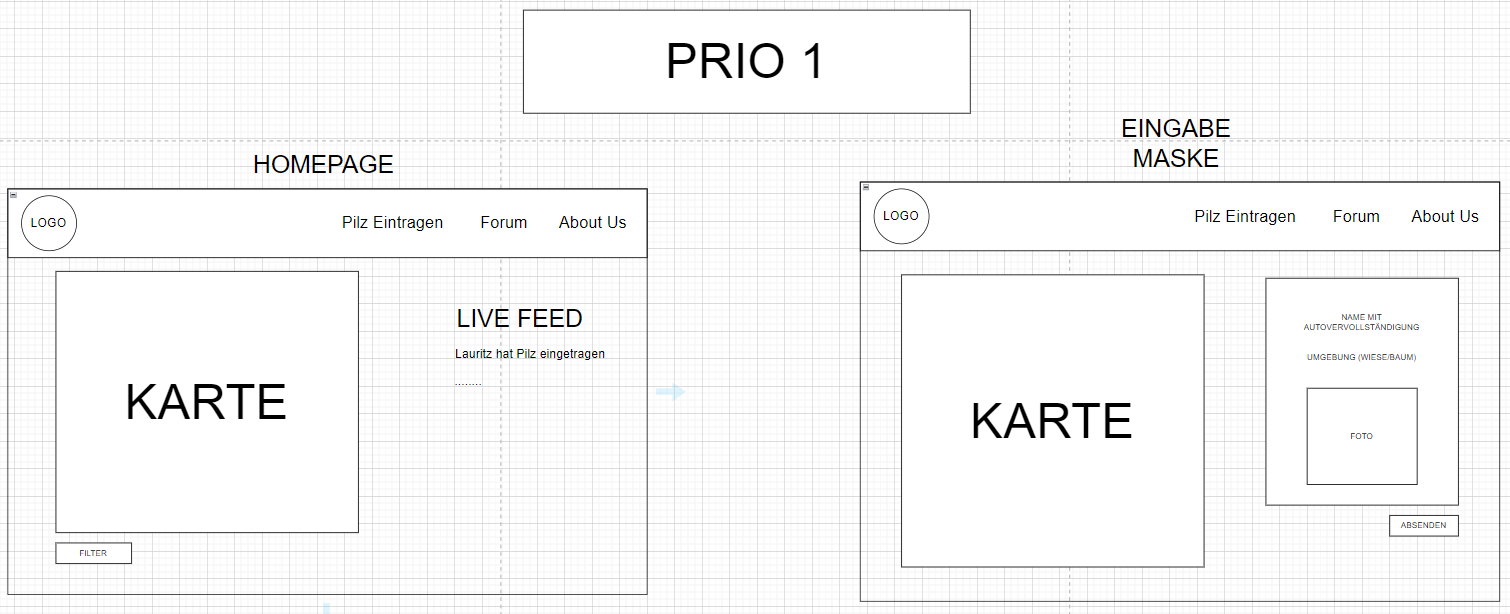
\includegraphics[width=\textwidth]{abbildungen/GuiEntwurfDrawio.jpg}
	\caption{Das Ergebnis des GUI Designs.}
	\label{fig:GUI_Entwurf}
\end{figure}

Nicht-funktionale Anforderungen wie Einfachheit, Benutzerfreundlichkeit und Responsive Design waren hierbei maßgebliche
Faktoren, an denen sich der Designprozess orientierte. Die Einfachheit der Benutzeroberfläche wurde als essenziell erachtet,
um die Nutzerführung intuitiv und zugänglich zu gestalten. So wurde jedes Element der GUI, sowie deren Anordnung, mit dem Ziel
entworfen, eine direkte und unkomplizierte Interaktion möglich zu machen. Benutzerfreundlichkeit stand ebenfalls im Vordergrund,
um sicherzustellen, dass Nutzer aller Erfahrungsstufen die Anwendung problemlos verwenden können. So gibt es keine überflüssigen
Elemente und die vorhandenen sind gut sichtbar und selbsterklärend. Die Anpassung an verschiedene Endgeräte durch ein Responsive
Design war ein weiterer kritischer Aspekt, der ebenfalls Berücksichtigung fand, da die Applikation höhst wahrscheinlich schon
während des Pilzesuchens verwendet wird. So wurde sich entschieden, bei schmaleren Bildschirmen die Karte anstatt auf der linken
Hälfte auf der oberen Hälfte des Bildschrimes anzuzeigen. Der Live-Feed, bzw. die Eingabemaske rutscht in diesem Fall direkt darunter.
So gewährleistet das Responsive Design, dass `ShroomScout' auf Smartphones gleichermaßen funktionell und ästhetisch ansprechend ist,
wie auf Desktops und Tablets.

\subsubsection{Frontend-Framework Entscheidung}

Nach der Gestaltung der GUI stand letztlich noch die Auswahl eines Frontend-Frame\-works an. Ein Frontend-Framework ist eine Sammlung
wiederverwendbarer Designvorlagen und Code-Snippets, die Entwicklern helfen, konsistente und effiziente Benutzeroberflächen zu
erstellen. Diese Frameworks bieten vorgefertigte Komponenten und Werkzeuge, die die Entwicklung beschleunigen und die Einhaltung
von Webstandards erleichtern.

Die Entscheidung fiel recht schnell auf Angular, hauptsächlich aufgrund von bereits vorhandenen Erfahrungen und aufgebautem
Basiswissen mit der Technologie. Obwohl andere Frontend-Frameworks wie React und Vue ebenfalls in Betracht gezogen wurden,
gab die Vertrautheit mit Angular den Ausschlag. React, bekannt für seine Flexibilität und Leistung, und Vue, geschätzt für
seine Einfachheit und leichtes Lernen, wären ebenfalls hervorragende Optionen für die Entwicklung moderner Webanwendungen gewesen.
Die Entscheidung für Angular basierte jedoch auf der spezifischen Projekterfahrung und dem Komfortniveau der Entwickler.

Darüber hinaus lassen sich weitere Vorteile von Angular, bzw. generell eines Frontend-Frameworks finden, welche den Entwicklungsprozess
des Frontends unterstützten:

\begin{itemize}

	\item
	      Angular überzeugt durch eine komponentenbasierte Architektur und dadurch modulare Herangehensweise bei der Entwicklung.
	      Jeder Baustein der Anwendung wird dabei in einer Komponente gekapselt, was Klarheit der Anwendungsstruktur fördert und die
	      Wiederverwendung dieser Komponenten möglich macht.

	\item
	      Die Bereitstellung umfangreicher Bibliotheken von eingebauten Funktionen und Diensten, wie Formularverwaltung, Routing oder
	      ein HTTP-Client, bietet durch die Vereinfachung der Entwicklung signifikante Vorteile.

	\item
	      Die Verwendung von TypeScript, welches JavaScript um starke Typisierung und objektorientierte Programmierkonzepte wie Klassen,
	      Interfaces und Dekoratoren erweitert, ermöglicht eine deutlich verbesserte Entwicklungserfahrung.

	\item
	      Angular ermöglicht durch seine umfangreiche Dokumentation und Community-Unterstützung eine effiziente Problemlösung und
	      Weiterentwicklung. Auch lassen sich dadurch zu den meisten Problemen sehr schnell Lösungen finden, was die Geschwindigkeit der
	      Entwicklung beschleunigt.

\end{itemize}

\documentclass[../main.tex]{subfiles}
%~1800 Worte
\begin{document}
\subsection{Uebergreifende Technologien} %Lauritz
\subsubsection{Git \& VSCode}
\subsubsection{Open Street Map}

\subsection{Datenbankloesung} %Tim
\subsubsection{SQLite}
\subsubsection{Tabellenstruktur}

\subsection{Backend Technologien} %Tim
\subsubsection{FastAPI mit Python}
\subsubsection{Uvicorn ASGI Server}

\subsection{Frontend Technologien} %Lauritz
\subsubsection{Angular mit Typescript, HTML \& CSS}
\subsubsection{Komponentenhierarchie}
\subsubsection{Messageflow \& RxJS}
\end{document}


\documentclass[../main.tex]{subfiles} % ~2200 Worte

\begin{document}

\subsection{Entwicklungsmethodik}

\subsubsection{Agile Arbeitsweise}

Die Agile Arbeitsweise repräsentiert eine revolutionäre Verschiebung in der Methodik der Softwareentwicklung, die zu Beginn des 21.
Jahrhunderts entstand. Ihre Ursprünge lassen sich auf das `Agile Manifesto' zurückführen, das von einer Gruppe von Softwareentwicklern
verfasst wurde. Das Manifest legt den Fokus auf Flexibilität, Kundenorientierung und die kontinuierliche Auslieferung von Software. Es
stellt einen Gegenentwurf zu den traditionellen, starren und plangetriebenen Entwicklungsmodellen dar, die sich oft als ineffizient in
der schnelllebigen und veränderlichen Welt der Softwareentwicklung erwiesen haben.

Die Agile Arbeitsweise umfasst verschiedene Prinzipien und Praktiken, die die enge Zusammenarbeit im Team, die Anpassungsfähigkeit an
Veränderungen, die kontinuierliche Verbesserung und die häufige Auslieferung von funktionierenden Softwareteilen betonen. Zu den
Kernprinzipien gehören die Priorisierung von Kundenbedürfnissen, die Arbeit in iterativen und inkrementellen Zyklen (Sprints),
Selbstorganisation und Cross-Funktionalität der Teams sowie die regelmäßige Reflexion zur Optimierung der Arbeitsprozesse.

Auf der Grundlage der agilen Prinzipien haben sich verschiedene Arbeitsweisen wie Scrum und Kanban entwickelt, die spezifische
Rahmenwerke und Methoden bieten, um Agile in der Praxis umzusetzen. Scrum fokussiert sich auf die Organisation der Teamarbeit in
Sprints mit festen Rollen (wie Product Owner und Scrum Master), Artefakten (wie Product Backlog und Sprint Backlog) und regelmäßigen
Meetings (Daily Scrum, Sprint Review, Sprint Retrospective). Kanban hingegen betont die Visualisierung der Arbeit durch ein Kanban-Board,
die Limitierung laufender Arbeiten und die kontinuierliche Lieferung, ohne feste Iterationen.

Die Vorteile der Agilen Arbeitsweise sind vielfältig. Sie ermöglicht eine höhere Reaktionsfähigkeit auf Kundenwünsche und Marktanforderungen,
führt zu einer verbesserten Produktqualität durch kontinuierliches Feedback und ermöglicht eine effizientere Ressourcennutzung durch adaptive
Planung. Darüber hinaus fördert sie eine stärkere Einbindung und Motivation der Teammitglieder, indem sie Eigenverantwortung und direkte
Kommunikation in den Vordergrund stellt.

Für das Projekt `ShroomScout' wurde sich aufgrund bereits vorhandener Arbeitserfahrungen für eine agile Herangehensweise entschieden. Die
Entscheidung basiert auf der Erkenntnis, dass agile Methoden eine flexible und effektive Rahmenstruktur bieten, um den Herausforderungen
und Dynamiken der Softwareentwicklung gerecht zu werden. Die Agilität ermöglicht es dem Team, schnell auf Änderungen zu reagieren, kontinuierlich
Wert zu liefern und dabei den Entwicklungsprozess stetig zu optimieren. Diese Erfahrungen und die Überzeugung von den Vorteilen agiler Prinzipien
führten zur Implementierung agiler Praktiken als grundlegende Entwicklungsstrategie für `ShroomScout', um ein hochwertiges, benutzerzentriertes
Produkt in einem kollaborativen und adaptiven Entwicklungsprozess zu realisieren.

\subsubsection{Software Kanban Board}

Software Kanban ist eine Methode des Lean Managements, die ursprünglich in der Produktion bei Toyota entwickelt wurde und mittlerweile weitreichende
Anwendung in der Softwareentwicklung findet. Das Kernstück dieser Methode ist das Kanban Board, ein visuelles Werkzeug zur Darstellung von Arbeitsabläufen.
Ein Kanban Board ist typischerweise in mehrere Spalten unterteilt, die verschiedene Phasen des Arbeitsprozesses repräsentieren, von `Zu tun' über `In Arbeit'
bis hin zu `Erledigt'. Jede Aufgabe, repräsentiert durch eine Karte (oder `Issue'), wird durch die Spalten bewegt, um ihren Fortschritt durch den Arbeitsprozess
zu visualisieren. Diese Methode unterstützt Teams dabei, den Arbeitsfluss zu optimieren, Engpässe zu identifizieren und die Effizienz zu steigern.

Im Rahmen des `ShroomScout'-Projekts wurde ein Kanban Board auf GitHub als Project implementiert. GitHub bietet die Möglichkeit, solche Boards direkt in den
Projektkontext zu integrieren. Beide Teammitglieder hatten Zugriff auf das Board, was eine flexible und transparente Zusammenarbeit ermöglichte. Die Nutzung
eines Kanban Boards auf GitHub erlaubte es dem Team, selbstständig Issues zu erstellen, diese entsprechenden Personen zuzuweisen und ihren Status zu aktualisieren,
sobald Aufgaben begonnen oder abgeschlossen wurden.

Ein wesentlicher Vorteil dieser Herangehensweise ist die Möglichkeit, in Git Commit Messages direkt auf Issues zu verweisen. Dies ermöglichte eine nahtlose
Nachverfolgbarkeit von Codeänderungen zu spezifischen Aufgaben und förderte ein tiefgreifendes Verständnis darüber, welche Änderungen aus welchem Grund
vorgenommen wurden. Diese Praxis erhöht die Codequalität und erleichtert die Fehlersuche und -behebung.

Die Anwendung eines Software Kanban Boards via GitHub brachte zahlreiche Vorteile für das `ShroomScout'-Projekt mit sich. Zu diesen Vorteilen zählten:

\begin{itemize}

	\item \textbf{Transparenz:}
	      Jedes Teammitglied hatte jederzeit einen vollständigen Überblick über den aktuellen Projektstatus, wer an welchen Aufgaben arbeitet und welche
	      Issues noch bearbeitet werden müssen. Diese Transparenz förderte das gemeinsame Verständnis und die Zusammenarbeit im Team, sowie das individuelle
	      Zeitmanagement.

	\item \textbf{Übersichtliche Planung:}
	      Die visuelle Darstellung des Arbeitsprozesses erleichterte die Priorisierung von Aufgaben und die Planung kommender Arbeitsschritte.
	      Engpässe und ungenutzte Ressourcen konnten schnell identifiziert und adressiert werden.

	\item \textbf{Flexibilität:}
	      Die Möglichkeit, Issues flexibel zwischen den Spalten zu verschieben, unterstützte das Team dabei, auf Veränderungen im Projektumfeld oder neue
	      Ideen für Anforderungen reagieren zu können, ohne den Überblick zu verlieren.

	\item \textbf{Verbesserte Kommunikation:}
	      Durch die Zuweisung von Aufgaben und die direkte Referenzierung von Issues in Commit Messages wurde die Kommunikation innerhalb
	      des Teams sowie die Dokumentation des Entwicklungsprozesses verbessert.

\end{itemize}

Insgesamt trug die Anwendung von Software Kanban und die Nutzung eines Kanban Boards auf GitHub maßgeblich zur Effizienz, Transparenz und Flexibilität des
Entwicklungsprozesses bei `ShroomScout' bei und stellte eine solide Basis für eine erfolgreiche Projektumsetzung dar.

\subsubsection{Anwendung von Scrum Artefakten \& Events}

Im Rahmen des `ShroomScout'-Projekts wurde eine angepasste Form der Scrum-Methodik angewendet, um die agile Entwicklung zu unterstützen. Scrum, eine der
prominentesten agilen Methoden, ist bekannt für seine strukturierte Herangehensweise an die Softwareentwicklung, die iterative Arbeit in Sprints, regelmäßige
Abstimmungsmeetings und eine klare Rollenverteilung innerhalb des Teams vorsieht. Eine zentrale Komponente von Scrum sind die täglichen Stand-up-Meetings, auch
als Daily Scrums bekannt, die dazu dienen, den Fortschritt zu überprüfen und den weiteren Arbeitsablauf effektiv zu koordinieren.

Für das Projekt wurde diese Praxis durch die Einführung eines täglichen 15-minütigen Anrufs, des Daily Calls, adaptiert. Diese kurzen, fokussierten Meetings
dienten als Plattform, um Aktualisierungen zu teilen, den Fortschritt zu diskutieren und Herausforderungen sowie die Planung für den kommenden Tag zu besprechen.
Trotz der Kürze waren diese Calls ausreichend, um eine kontinuierliche Abstimmung zwischen den Teammitgliedern zu gewährleisten und sicherzustellen, dass alle
auf dem gleichen Stand sind.

Die Kombination des Daily Calls mit dem Einsatz eines Kanban Boards auf GitHub erwies sich als besonders effektiv. Während das Kanban Board eine kontinuierliche
visuelle Übersicht über den Status aller Aufgaben bot, ermöglichten die Daily Calls eine dynamische Anpassung an Veränderungen und die sofortige Klärung von
Fragen. Diese Synergie förderte nicht nur die Transparenz und Flexibilität im Entwicklungsprozess, sondern trug auch dazu bei, die Prinzipien der agilen Entwicklung,
wie schnelle Anpassungsfähigkeit an Veränderungen und verbesserte Kommunikation, effektiv umzusetzen.

Die Anwendung dieser angepassten Scrum-Methodik im `ShroomScout'-Projekt illustriert, wie agile Praktiken an die spezifischen Bedürfnisse und Rahmenbedingungen
eines Projekts angepasst werden können. Die täglichen Calls stärkten die Teamdynamik und förderten eine Kultur der Offenheit und des kontinuierlichen Lernens.
In Kombination mit dem Kanban Board ermöglichte diese Vorgehensweise eine agile, reaktionsfähige und effiziente Projektarbeit, die maßgeblich zum erfolgreichen
Abschluss von `ShroomScout' beitrug.

\subsection{Herausforderungen \& Bewaeltigungsstrategien} % Tim

\subsubsection{Open Streetmap Datenbank}

\subsection{Qualitaetssicherung \& Testing}

\subsubsection{Anwendung von Clean Code Prinzipien}

Clean Code bezeichnet eine Sammlung von Prinzipien und Praktiken für die Softwareentwicklung, die darauf abzielen, den Quellcode lesbar, verständlich und wartbar
zu gestalten. Außerdem führt die Einhaltung von Clean Code Prinzipien zu einer höheren Codequalität und erleichtert die Zusammenarbeit in Teams. Vorteile umfassen
in der Theorie unter anderem die Reduzierung von Fehlern, eine effizientere Einarbeitung neuer Teammitglieder und eine gesteigerte Produktivität bei der Weiterentwicklung
der Software. Folgende grundlegende Prinzipien des Clean Code wurden im Projekt berücksichtigt:

\begin{itemize}

	\item \textbf{Klarheit und Verständlichkeit:}
	      Der Code sollte so geschrieben sein, dass er auch von anderen Entwicklern leicht verstanden werden kann. Dies beinhaltet die Verwendung aussagekräftiger
	      Namen für Variablen, Funktionen und Klassen sowie eine klare Strukturierung des Codes. Ein Beispiel dafür findet sich etwa in der Eingabemaskenkomponente
	      (`register.component.ts'):

	      \begin{verbatim}
          // Schlecht
          protected t: string = 'Pilzdaten angeben:';
          protected env: string[] = ['Wiese', 'Eiche', 'Buche'];
          protected sEnv: string = '';

          // Gut
          protected title: string = 'Pilzdaten angeben:';
          protected environments: string[] = ['Wiese', 'Eiche', 'Buche'];
          protected selectedEnvironment: string = '';
        \end{verbatim}

	\item \textbf{Kurze Funktionen und Klassen:}
	      Funktionen und Klassen sollten eine einzige Aufgabe erfüllen und möglichst kurz gehalten werden. Dies trägt zur Lesbarkeit und Wiederverwendbarkeit bei.
	      Ein Beispiel stellt die Kartenkomponente (`map.component.ts') dar:

	      \begin{verbatim}
          ngOnInit() {
            this.initializeMap();
            this.handleMapClicks();
          }
        \end{verbatim}

	      Der Inhalt der beiden Methoden hätte auch innerhalb der `ngOnInit()' Methode, welche von Angular beim initialisieren der Komponente aufgerufen wird,
	      eingefügt werden können. Dies hätte jedoch zu einer sehr langen und unüberischtlichen `ngOnInit()' Methode geführt.

	\item \textbf{Vermeidung von Code-Duplikationen:}
	      Jedes Codefragment sollte eine eindeutige, unmissverständliche und einmalige Funktion innerhalb des Systems haben. Das wird zum Beispiel bei der Einbindung
	      der Kartenkomponente deutlich. Da diese immer zu sehen ist, wird sie auch nur einmal in der `app.component.ts' eingebunden. Lediglich der Teil daneben ändert
	      sich in Bezug auf die URL.

	\item \textbf{Verwendung von Kommentaren:}
	      Kommentare sollten genutzt werden, um die Intention hinter dem Code zu erklären, nicht um zu beschreiben, was der Code tut. Der Code selbst sollte durch
	      seine Klarheit überzeugen. Dies wird ebenfalls in der Kartenkomponente deutlich. Da in der Methode die Karte bei bestimmten Koordinaten initialisiert wird,
	      stellt der Kommentar klar, dass es sich hierbei um Berlin handelt, nicht etwa wie das Laden genau funktioniert.

	      \begin{verbatim}
          /**
          * Initializes the leaflet map to Berlin's coordinates
          * and loads the actual map tiles from OSM.
          */
          private initializeMap(): void {...}
        \end{verbatim}

\end{itemize}

Die Anwendung von Clean Code Prinzipien im `ShroomScout'-Projekt trug wesentlich zur Qualitätssicherung und zur Effizienz der Softwareentwicklung bei. Durch
die konsequente Umsetzung dieser Prinzipien konnte ein Code erstellt werden, der nicht nur funktional zuverlässig ist, sondern auch eine hohe Lesbarkeit und
Wartbarkeit aufweist.

\subsubsection{Unit Tests}

In der Softwareentwicklung ist eine strukturierte Testhierarchie essenziell, um die Qualität und Zuverlässigkeit von Softwareprodukten zu gewährleisten. Diese
Hierarchie beginnt typischerweise mit Unit Tests, gefolgt von Integrationstests, Systemtests bis hin zu Akzeptanztests. Jede Testebene adressiert unterschiedliche
Aspekte der Software und hilft dabei, Fehler und Probleme frühzeitig im Entwicklungsprozess zu identifizieren.

Unit Tests stellen die Basis dieser Hierarchie dar und fokussieren sich auf die Überprüfung der kleinsten testbaren Teile einer Anwendung, in der Regel einzelne
Funktionen oder Methoden. Durch die Isolation spezifischer Codeabschnitte ermöglichen Unit Tests die Überprüfung der Funktionalität und Korrektheit einzelner
Komponenten unabhängig vom restlichen System.

Die Vorteile von Unit Tests sind vielfältig:

\begin{itemize}

	\item \textbf{Frühe Fehlererkennung:}
	      Unit Tests helfen, Fehler und Probleme bereits in der Entwicklungsphase zu erkennen, bevor sie tiefgreifende Auswirkungen auf das Gesamtsystem haben.

	\item \textbf{Dokumentation:}
	      Sie dienen als lebendige Dokumentation des Codes, indem sie dessen erwartetes Verhalten beschreiben.

	\item \textbf{Designverbesserung:}
	      Die Notwendigkeit, Codeeinheiten isoliert zu testen, fördert saubere und lose gekoppelte Codearchitekturen.

\end{itemize}

Für das Projekt `ShroomScout' wurde sich ausschließlich für die Implementierung von Unit Tests entschieden. Diese Entscheidung basiert auf der Erkenntnis,
dass umfangreichere Testformen wie Integrationstests oder Performance Tests ohne eine Produktionsumgebung und angesichts der ständigen Weiterentwicklung des
Projekts nur begrenzten Mehrwert bieten würden. Unit Tests hingegen er\-mög\-lich\-en eine effektive und effiziente Überprüfung der Kernfunktionalitäten von
`ShroomScout' und unterstützen eine agile Entwicklungsmethodik.

\textit{Codebeispiele zur Verdeutlichung der Zwecke von Unit Tests:}

\begin{verbatim}

...

\end{verbatim}

Die Anwendung von Unit Tests in `ShroomScout' spielte eine zentrale Rolle in der Qua\-li\-täts\-sich\-e\-rung, indem sie die Zuverlässigkeit einzelner
Funktionen und Methoden kontinuierlich überprüfte. Dies trug wesentlich zur Stabilität und Wartbarkeit des Projekts bei und stellte sicher, dass auch bei
zukünftigen Erweiterungen und Anpassungen die Integrität der Anwendung gewahrt bleibt.

\end{document}

\documentclass[../main.tex]{subfiles}
%1000 Worte, Tim
\begin{document}
\subsection{Anforderungskonformität der Applikation}
Das wichtigste Kriterium für gute Software ist Anforderungskonformität, im folgenden werden die Anforderungen den Ergebnissen gegenübergestellt:

\subsubsection{Funktionale Anforderungen}

\begin{itemize}

	\item \textbf{Anforderung: Registrieren eines Pilzfunds}
	      Der User muss die Möglichkeit haben einen neuen Pilzfund, über eine Eingabemaske im Frontend zu registrieren.
		  Diese Eingabemaske soll eine automatische Vervollständigung der Eingabe anbieten und soll bereits validieren ob die Eingabe einem gültigen
		  Wert entspricht. Die in die Eingabemaske einzugebenden Daten sind die Art des Pilzes sowie die Umgebung in der er gefunden wurde.
		  Erst wenn ein Marker für den Standort auf der Karte gesetzt und sowohl für Art und Umgebung des Pilzes valide Werte eingetragen wurden, soll es 
		  möglich sein den Eintrag zu speichern, davor soll der Button zum registrieren ausgegraut sein.
          
    \item \textbf{Umsetzung: Registrieren eines Pilzfunds}
          Die Eingabemaske wurde entsprechend der Anforderungen umgesetzt. 
          Die Validation der vom User eingegeben Werte wurde mit Hilfe von Angular FormControl und der Angular Materials Komponente Autocomplete umgesetzt.

	\item \textbf{Anforderung: Anzeigen eines Live Feeds}
	      Es soll auf der Startseite einen Livefeed geben in dem die letzten Pilzfunde geben. 
		  Aus dem Livefeed sollen Art und Umgebung der zuletzt registrierten Pilze hervorgehen

    \item \textbf{Umsetzung: Anzeigen eines Live Feeds}
          Der Live Feed wurde mit Hilfe eines Angular Services und einer Angular Materials Komponente umgesetzt. 

	\item \textbf{Anforderung: Anzeige der registrierten Pilze}
		  Die registrierten Pilze sollen auf einer Openstreetmap Karte als Marker angezeigt werden.
		  Wenn die Marker angeklickt werden sollen zusätzliche Informationen wie die Art des Pilzes angezeigt werden.

	\item \textbf{Umsetzung: Anzeige der registrierten Pilze}
		  Die registrierten Pilze werden anhand ihrer Längen und Breitendaten in der Datenbank gespeichert.
          Beim Laden der Seite werden die Information Namen, Umgebung, Längengrad und Breitengrad von einem Angular Service beim Backend abgefragt, anschließend ans Frontend gesendet
          und als Marker auf der Karte angezeigt.

	\item \textbf{Anforderung: Navbar}
	      Die Navbar soll die Navigation der Seite ermöglichen und die Möglichkeit bieten, die Eingabemaske zum Registrieren eines Pilzes zu öffnen, sowie zur Startseite zurückzukehren.
		  Die Navbar soll blau sein und am linken Bildschirmrand das Shroomscout Logo beinhalten.

    \item \textbf{Umsetzung: Navbar}
	      Die Navbar wurde mit Hilfe der Angular Material Navbar Komponente implementiert und ermöglicht den Zugriff auf alle Teile des Frontends.
          Die Navbar ist blau und beinhaltet das Shroomscout Logo am linken Bildschirmrand.

	\item \textbf{Anforderung: Design}
	      Um eine einheitliche Erfahrung zu schaffen und die Wartung zu erleichtern, sollen primär Komponenten der von Google verwalteten Angular Materials Library verwendet werden.

    \item \textbf{Umsetzung: Design}
          Bis auf die Karte, wurde das Design der Website ausschließlich mit Angular Components Komponenten erstellt.
\end{itemize}

\subsubsection{}

\subsection{Ausblick auf zukuenftige Entwicklungen}
Die Entwicklung einer Software ist nie endgültig abgeschlossen, es existieren stets Optimierungspotentiale und potentielle weitere Features.
Würde die Entwicklung von Shroomscout unmittelbar weitergeführt werden, wären die folgenden Punkte die unmittelbaren Verbesserungspotenziale

\begin{itemize}

    \item \textbf{Performanteres Datenbanksystem}
        Die Verwendung eines performanteren serverbasierten Datenbanksystem bildet das Fundament für weitere Optimierungen, da die aktuelle Lösung nicht für userintensive
        Produktivanwendungen ausgelegt ist und daher bei der Skalierung der Software schnell zum Flaschenhals werden würde. Der Migrationsaufwand auf ein System wie MySQL oder PostgreSQL
        wäre, des Weiterem mit verhältnismäßig geringem Aufwand verbunden, da solange die Tabellenstruktur übernommen wird, die nötigen Anpassungen am Code verhältnismäßig klein sind. 

	\item \textbf{Containerrisierung \& Microservices}
	    Die Software folgt aktuell dem Server-Client-Muster und ist darauf ausgelegt unmittelbar auf einem System zu Laufen.
        Zur Erleichterung des Deployments und Erhöhung der Skalierbarkeit, ist es sinnvoll Container Virtualisierungslösungen, wie beispielsweise Docker oder Podman zu nutzen.
        In diesem Rahmen wäre ebenfalls eine Anpassung der Systemarchitektur hin zu Microservices sinnvoll, bei diesem Ansatz wird die Applikation in viele Microservices aufgespalten,
        die jeweils eine oder wenige Aufgaben erfüllen und unabhängig von einander laufen. Die Vorteile dieses Architekturansatz liegt ebenfalls in der erhöhten Skalierbarkeit, jedoch
        bietet er auch erleichterte Fehlerfindung durch getrennt laufende Services, die individuell getestet werden können.
        
    \item \textbf{Implementierung von Validierungen}
        Eine wichtige Optimierung im Hinblick auf die Sicherheit der Applikation ist die Implementierungen von Validierungen für User Input und Anfragen an das Backend.
        Die aktuellen Validierungen, verhindern nur eine versehentliche eingabe ungültiger Werte durch den Nutzer und SQLinjection Attacken. Anfragen das Backend hingegen werden
        im Moment nicht validiert, was potentiell zu Sicherheitslücken führen kann. Die Implementierung dieser Validierungen ist mit verhältnismäßig geringem Aufwand verbunden,
        es besteht jedoch das Risiko, dass nicht alle Fälle abgedeckt werden. Des Weiteren ist es im produktiven Einsatz wichtig, Techniken wie Ratelimiting zu implementieren um 
        DDOS Attacken vorzubeugen.
        
    \item \textbf{Usersystem}
        Im Moment funktioniert Shroomscout weitestgehend anonym, ein Nutzer muss sich nicht authentifizieren um die Software zu nutzen. Dies hat einige Vorteile, nicht zuletzt die
        Vereinfachte Umsetzung von Datenschutzrichtlinien bei minimaler Erhebung von Nutzerdaten, jedoch bringt die Implementierung eines Usersystems viele Vorteile mit sich.
        User könnten Präferenzen oder Filter speichern und eine zwingende Registrierung zur Nutzung der Anwendung kann Helfen, Missbrauch der Plattform zu verhindern.

    \item \textbf{Reimplementierung des Backendcodes}
        Das Backend wurde in Python implementiert, maßgebliche Kriterien für diese Entscheidung waren die Einfachheit und das breite Angebot von Ressourcen für die Programmiersprache.
        Python ist jedoch, verglichen mit anderen Programmiersprachen, nicht sehr performant und ressourceneffizient. Daher kann es sinnvol

\end{itemize}



\end{document}


\end{document}
